% The first question that we want to solve is what data should we collect in order to build a robot that can draw with humans? Inspired by drawing sessions created by Bob Ross, we have considered painting with robots and experimented briefly with oil painting on canvas with a Franka robot, but precise execution of brush strokes and the technical details surrounding manipulating brushes to create the desire scene are even very difficult for humans, and the focus of our research is to make a step towards human-robot collaboration on tasks, we do not want to be side-tracked by difficulties around robot control, which in itself is an extremely interesting problem that we wish to explore another time. 
\begin{figure*}[!htb]
\centering
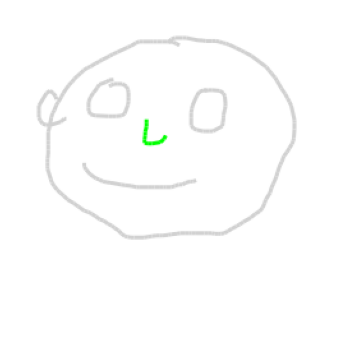
\includegraphics[width=0.3\linewidth]{future/future_nose_variety_392.png}  
\caption{.}
\label{results.hookNose}
\end{figure*}
There are many creative use of language in our dataset, and in follow-up work, we want to investigate what categories of creative usage are there and quantify how many cases are in each category. 
Most of our current characterization of the dataset are based on looking through a few examples in the datasets (there are a total of 11K!).
Since we did not put limits on what language annotators could use during data collection, such as specifying a fixed list of attributes for the annotators to choose from, the dataset contains a variety of ways of describing the same concept. For example, for a nose that looks similar to the one in Figure \ref{results.hookNose}, annotators describe it as \textit{hook-shaped}, \textit{c-shaped}, \textit{inverted j}, \textit{curved}, etc. We believe that this case is not the only one, and we want to quantify the diversity. In this way, we can evaluate how a multi-modal embedding space, such as the CLIP joint embedding, captures these relationships. Is the feature vector of the sketch collinear with the word features of every one of these words?          

So far, we have observed that face and angel sketches share many visual concepts. These could be related to length (\textit{long,short}), size (\textit{big,small}), geometry (\textit{circular, triangular}), direction (\textit{horizontal, vertical}), and many more. We want to evaluate more thoroughly which concepts are shared and which ones are unique to each category. In this way, we can understand better the chalenges around generalizing CLIP to unseen categories, indicated by results in Section \ref{results.acc}. 



% Text representation. 
% We have RNN to model the sequence of strokes. 
% Can we still use RNN to model the sequence of words? Does the length of the sentence matter? If we only have adjectives, how can we effectively model these words? 
% What are methods that can model the semantics of these words alone? 
% Where can we find existing representations of these words? How are traditional text-image synthesis methods modeling the words? 
% Reed et al. [28] obtain the text encoding of a textual description by using a pre-trained character-level convolutional recurrent neural network (char-CNN-RNN). The char-CNN-RNN is pretrained to learn a correspondence function between text and image based on the class labels. 
